\documentclass[a4paper,11pt]{article}

%%%%%%%%%%%%%%%%%%%%%%%%%%%%%%%%%%%%%%%%%%%%%%%%%%%%%%%%%%%%%%%%%%%%%%%%
% Paquetes utilizados
%%%%%%%%%%%%%%%%%%%%%%%%%%%%%%%%%%%%%%%%%%%%%%%%%%%%%%%%%%%%%%%%%%%%%%%%

% Gráficos complejos
\usepackage{graphicx}
\usepackage{caption}
\usepackage{subcaption}
\usepackage{placeins}

% Soporte para el lenguaje español
\usepackage{textcomp}
\usepackage[utf8]{inputenc}
\usepackage[T1]{fontenc}
\DeclareUnicodeCharacter{B0}{\textdegree}
\usepackage[spanish]{babel}

% Código fuente embebido
\usepackage{listings}
\usepackage{courier}

% PDFs embebidos para el apéndice
\usepackage{pdfpages}

% Matemáticos
\usepackage{amssymb,amsmath}

% Tablas complejas
\usepackage{multirow}

% Formato de párrafo
\setlength{\parskip}{1ex plus 0.5ex minus 0.2ex}

% Formato de listados de código
\lstset{
  basicstyle=\footnotesize\ttfamily,
  numberstyle=\tiny,
  numbersep=5pt,
  tabsize=2,
  extendedchars=true,
  breaklines=true,
  keywordstyle=\color{red},
  frame=b,
  stringstyle=\color{white}\ttfamily,
  showspaces=false,
  showtabs=false,
  xleftmargin=17pt,
  framexleftmargin=17pt,
  framexrightmargin=5pt,
  framexbottommargin=4pt,
  showstringspaces=false
}
\usepackage{caption}
\DeclareCaptionFont{white}{\color{white}}
\DeclareCaptionFormat{listing}{\colorbox[cmyk]{0.43, 0.35, 0.35,0.01}{\parbox{\textwidth}{\hspace{15pt}#1#2#3}}}
\captionsetup[lstlisting]{format=listing,labelfont=white,textfont=white, singlelinecheck=false, margin=0pt, font={bf,footnotesize}}

%%%%%%%%%%%%%%%%%%%%%%%%%%%%%%%%%%%%%%%%%%%%%%%%%%%%%%%%%%%%%%%%%%%%%%%%
% Título
%%%%%%%%%%%%%%%%%%%%%%%%%%%%%%%%%%%%%%%%%%%%%%%%%%%%%%%%%%%%%%%%%%%%%%%%

% Título principal del documento.
\title{\textbf{Hiposoft}}

% Información sobre los autores.
\author{
  Andrés Gastón Arana, \textit{P. 86.203}                          \\
  Sergio Matías Piano, \textit{P. 85.191}                          \\
  Diego Martín Costa, \textit{P. 78.189}                           \\
  \normalsize{1er. Cuatrimestre de 2013}                           \\
  \normalsize{75.15 - Bases de datos}                              \\
  \normalsize{Facultad de Ingeniería, Universidad de Buenos Aires}
}
\date{}

%%%%%%%%%%%%%%%%%%%%%%%%%%%%%%%%%%%%%%%%%%%%%%%%%%%%%%%%%%%%%%%%%%%%%%%%
% Documento
%%%%%%%%%%%%%%%%%%%%%%%%%%%%%%%%%%%%%%%%%%%%%%%%%%%%%%%%%%%%%%%%%%%%%%%%

\begin{document}

% ----------------------------------------------------------------------
% Top matter
% ----------------------------------------------------------------------
\thispagestyle{empty}
\maketitle

\begin{abstract}

  Este informe sumariza el desarrollo del trabajo práctico de la materia Bases
  de Datos (75.15) dictada en el primer cuatrimestre de 2013 en la Facultad de
  Ingeniería de la Universidad de Buenos Aires. El mismo consiste en el
  modelado de datos de un software de administración de eventos hípicos en los
  hipódromos de la provincia de Buenos Aires, cuyos requisitos fueron extraídos
  de un caso de estudio real.

\end{abstract}

\clearpage

% ----------------------------------------------------------------------
% Tabla de contenidos
% ----------------------------------------------------------------------
\tableofcontents
\clearpage


% ----------------------------------------------------------------------
% Desarrollo
% ----------------------------------------------------------------------
\part{Desarrollo}

\section{Metodología y desarrollo}

Primeramente se analizó el enunciado entregado desarrollando un diagrama de
entidad-interrelación inicial plasmando el resultado del análisis.
Posteriormente se refinó el mismo al realizar una investigación de las
características del dominio del problema a resolver; particularmente, se
investigó en publicaciones hípicas de diversa procedencia acerca de las
diferentes relaciones entre jockeys, cuidadores y entrenadores con los studs
que a los que pertenecen los equinos, de manera de poder representar fielmente
en el diagrama las características de dichas relaciones.

Una vez completado y validado el diagrama de entidad interrelación, se
confeccionó el diccionario de datos, cuya elaboración fue trivial considerando
la existencia de dicho diagrama.

Posteriormente, se trabajó en el modelo relacional correspondiente al problema
relevado, mapeando cuidadosamente cada una de las entidades e interrelaciones a
las tablas. Se realizó en este caso también sucesivas aproximaciones al
diagrama final que se presenta en la sección correspondiente de este informe,
analizando las diversas estrategias de mapeo disponibles en cada caso y
seleccionando la más adecuada.

Finalmente, con el modelo relacional completo, se confeccionó un script SQL que
crea las tablas y restricciones correspondientes a dicho modelo utilizando el
subconjunto de instrucciones DDL del lenguaje.

\section{Modelo de entidad-interrelación} \label{sec:der}

\subsection{Hipótesis}

En la confección del diagrama se tomaron como verdaderas las siguientes
hipótesis, confirmadas en la investigación realizada sobre el dominio en
publicaciones hípicas diversas:

\begin{enumerate}

  \item Los cuidadores y entrenadores trabajan sobre varios equinos al mismo
    tiempo. Cada cuidador y entrenador puede estar trabajando sobre diferentes
    equinos en un momento dado, aunque cada equino posee únicamente un cuidador
    y un entrenador.

  \item Diferentes jockeys pueden correr con diferentes equinos. Cada equino
    participa de una carrera con un jockey particular, pero eso no significa
    que en posteriores carreras deba seguir participando con el mismo jockey.
    Cada jockey puede participar en diferentes carreras con diferentes equinos.

  \item Tanto cuidadores y entrenadores como jockeys no pertenecen a ningún
    stud en particular. El stud únicamente posee los equinos que le
    corresponden. Nada impide que un jockey participe en diferentes carreras
    con equinos de diferentes studs. Lo mismo es cierto para cuidadores y
    entrenadores, que pueden trabajar con equinos de distintos studs.

  \item Cada encuentro programado se realiza en su totalidad a lo largo de un
    único día.

\end{enumerate}

\subsection{Diagrama de entidad-interrelación}

En la figura \ref{fig:der} se incluye el diagrama de entidad-interrelación
final desarrollado para representar el dominio modelado cuyo relevamiento se
detalla en el enunciado.

\begin{figure}[h!t]
  \centering
  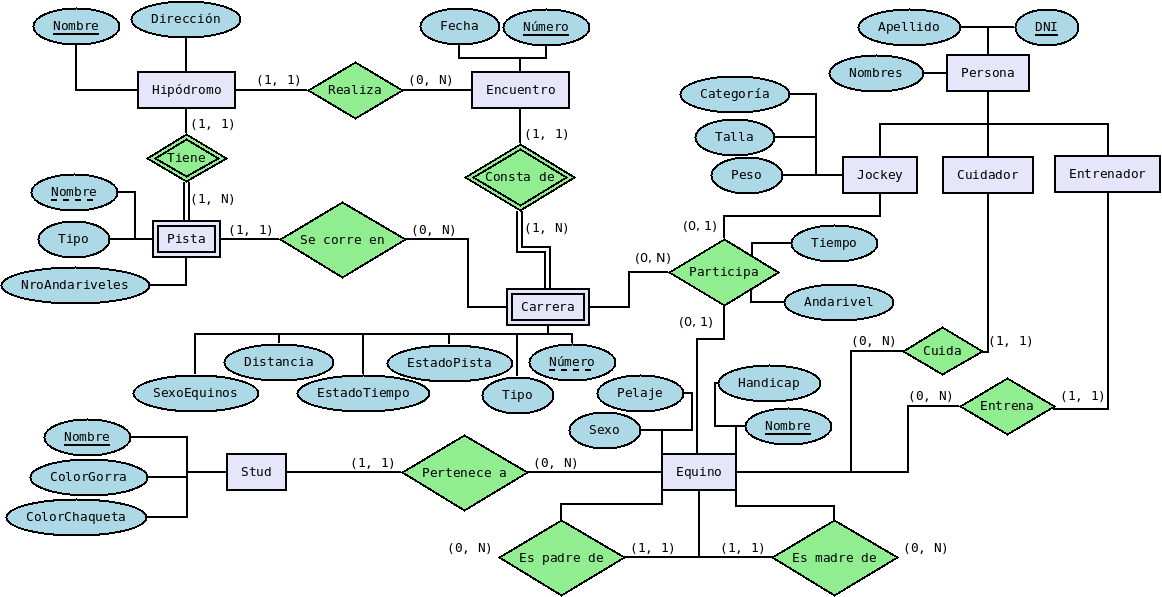
\includegraphics[width=1.50\textwidth, angle=90]{build/images/der.png}
  \caption{Diagrama de entidad-interrelación} \label{fig:der}
\end{figure}

\FloatBarrier

\subsection{Restricciones adicionales}

Las siguientes restricciones adicionales se detallan a continuación por
pertenecer al modelado de entidad-interrelación. No están representadas en el
diagrama dado que su inclusión agregaba complejidad adicional sobre en la
figura que consideramos innecesaria.

\begin{enumerate}

  \item La fecha del encuentro es única entre todos los encuentros.

  \item Cada caballo puede participar únicamente en una carrera por encuentro.
    Los jockeys pueden participar en cuantas carreras se quiera, en cada una de
    ellas con diferentes equinos.

\end{enumerate}

\section{Diccionario de datos}

[TODO: Definir el formato]

\section{Modelo relacional}

\subsection{Diagrama relacional}

En la figura \ref{fig:relacional} se incluye un diagrama representativo del
modelo relacional desarrollado para el modelo de entidad-interrelación
detallado en la sección \ref{sec:der}.

\begin{figure}[h!t]
  \centering
  \includegraphics[width=1.60\textwidth, angle=90]{build/images/rel.png}
  \caption{Modelo relacional} \label{fig:relacional}
\end{figure}

\FloatBarrier

\subsection{Scripts de creación}

A continuación se incluyen los scripts de creación de las tablas del modelo
relacional para ser ejecutado en un sistema de bases de datos que interprete
SQL, particularmente las instrucciones DDL de dicho lenguaje.

\lstinputlisting{scripts/hiposoft_schema.sql}

\clearpage

\part{Apéndice}
\appendix

\section{Enunciado original}\label{sec:enunciado}
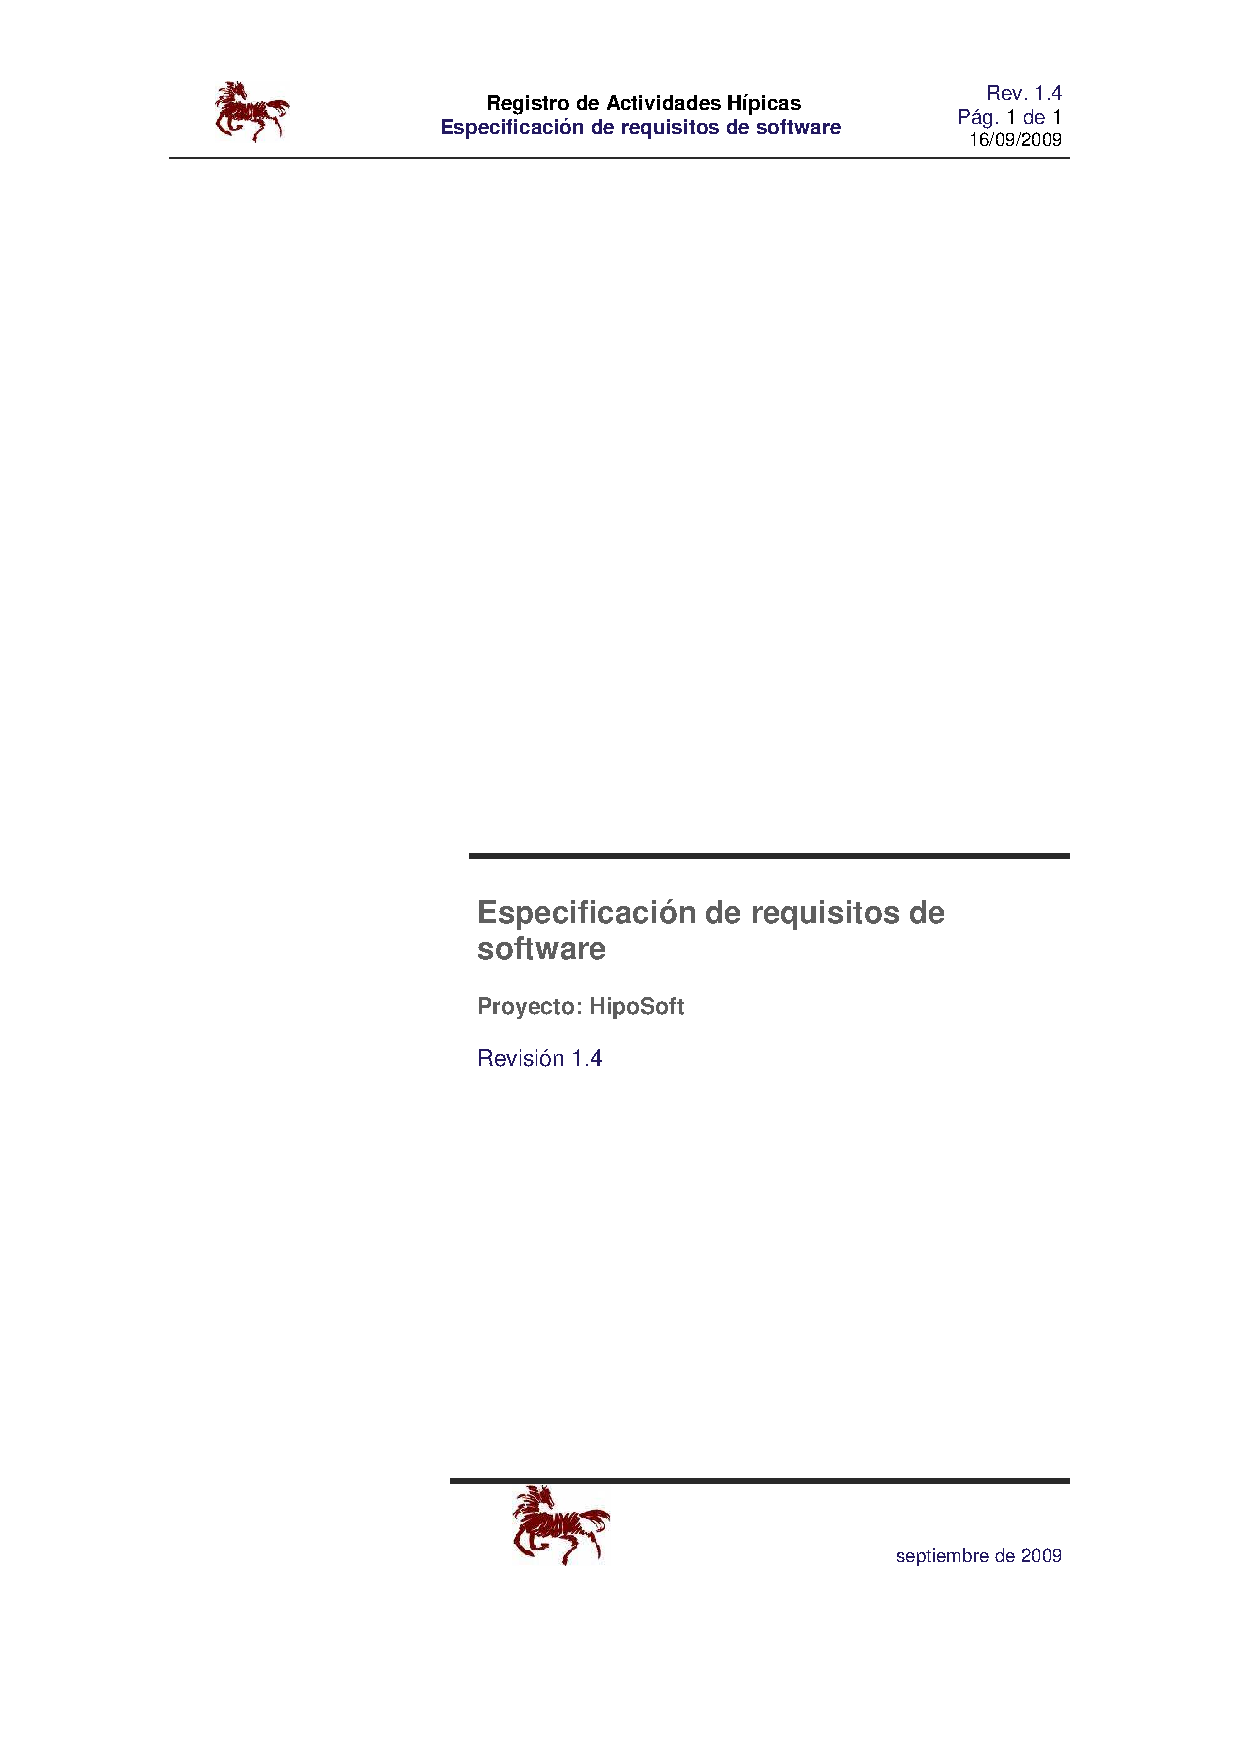
\includepdf[pages={-}, frame=true, pagecommand={}, noautoscale=true, scale=0.7]{enunciado.pdf}

\end{document}

